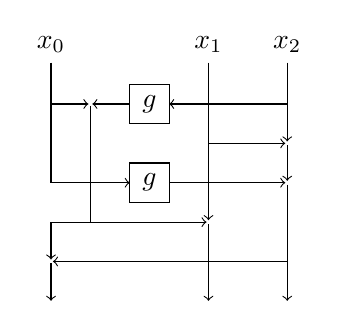
\begin{tikzpicture}[xscale=0.5,yscale=0.5]
  % nodes
  \draw (-2, 0.5) node (x0) {$x_0$} ;
  \draw ( 2, 0.5) node (x1) {$x_1$} ;
  \draw ( 4, 0.5) node (x2) {$x_2$} ;
  \draw (-1, -1) node[inner sep=0] (add0) {$\boxplus$} ;
  \draw ( 4, -2) node[inner sep=0] (add1) {$\boxplus$} ;
  \draw ( 4, -3) node[inner sep=0] (add2) {$\boxplus$} ;
  \draw ( 2, -4) node[inner sep=0] (add3) {$\boxplus$} ;
  \draw (-2, -5) node[inner sep=0] (add4) {$\boxplus$} ;
  \draw (0, -1.5) rectangle (1, -0.5) node [pos=0.5] {$g$} ;
  \draw (0, -3.5) rectangle (1, -2.5) node [pos=0.5] {$g$} ;

  % arrows
  \draw (x0) -- (-2, -3) ;
  \draw[->] (-2, -1) -- (add0) ;
  \draw (add0) -- (-1, -4) ;
  \draw[->] (x1) -- (add3) ;
  \draw[->] (x2) -- (add1) ;
  \draw[->] (4, -1) -- (1, -1) ;
  \draw[->] (0, -1) -- (add0) ;
  \draw[->] (2, -2) -- (add1) ;
  \draw[->] (add1) -- (add2);
  \draw[->] (-2, -3) -- (0, -3) ;
  \draw[->] (1, -3) -- (add2) ;
  \draw[->] (-1, -4) -- (add3) ;
  \draw[->] (-1, -4) -- (-2, -4) -- (add4) ;
  \draw[->] (4, -5) -- (add4) ;
  \draw[->] (add2) -- ( 4, -6) ;
  \draw[->] (add3) -- ( 2, -6) ;
  \draw[->] (add4) -- (-2, -6) ;
\end{tikzpicture}
